\documentclass[10pt]{article}
\usepackage[utf8]{inputenc}
\usepackage[T1]{fontenc}
\usepackage{graphicx}
\usepackage[export]{adjustbox}
\graphicspath{ {./images/} }
\usepackage{amsmath}
\usepackage{amsfonts}
\usepackage{amssymb}
\usepackage[version=4]{mhchem}
\usepackage{stmaryrd}

\title{PHYSICS }

\author{}
\date{}


\begin{document}
\maketitle
27th Jan Shift - 1

\section*{SECTION-A}
\begin{enumerate}
  \item Which among the following is forward biased:
\end{enumerate}

(1)

\begin{center}
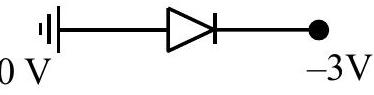
\includegraphics[max width=\textwidth]{2024_03_08_77386ce5bfd05109325bg-01(2)}
\end{center}

(2)

\begin{center}
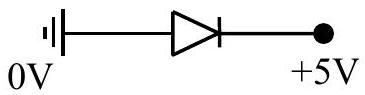
\includegraphics[max width=\textwidth]{2024_03_08_77386ce5bfd05109325bg-01(1)}
\end{center}

(3)

\begin{center}
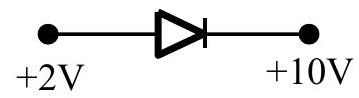
\includegraphics[max width=\textwidth]{2024_03_08_77386ce5bfd05109325bg-01(3)}
\end{center}

(4)

\begin{center}
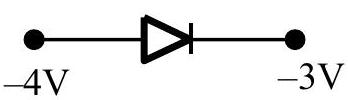
\includegraphics[max width=\textwidth]{2024_03_08_77386ce5bfd05109325bg-01}
\end{center}

Ans. (1)

Sol. Basic theory.

\begin{enumerate}
  \setcounter{enumi}{1}
  \item A uniform and homogeneous rod has resistance R. If rod is cut into 5 equal parts and connected in parallel find equivalent resistance?
\end{enumerate}

Ans. $\frac{\mathrm{R}}{25}$

Sol.\\
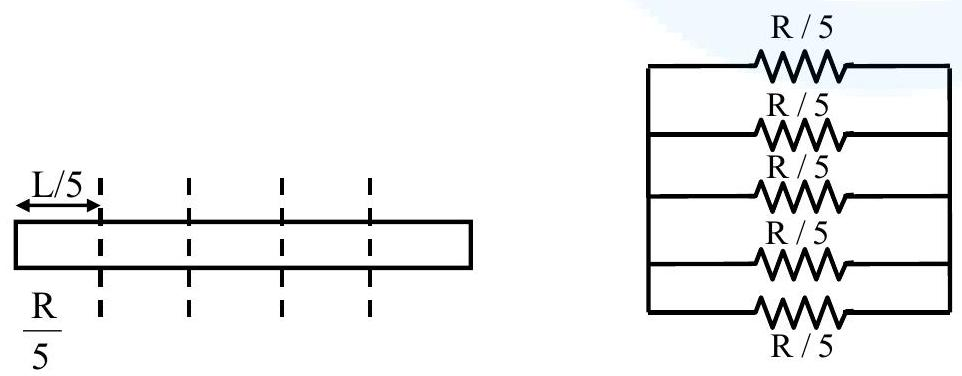
\includegraphics[max width=\textwidth, center]{2024_03_08_77386ce5bfd05109325bg-01(4)}

$\Rightarrow \quad \frac{\mathrm{R}}{25}$ Answer


\end{document}